% Options for packages loaded elsewhere
\PassOptionsToPackage{unicode}{hyperref}
\PassOptionsToPackage{hyphens}{url}
\PassOptionsToPackage{dvipsnames,svgnames,x11names}{xcolor}
%
\documentclass[
  letterpaper,
  DIV=11,
  numbers=noendperiod,
  oneside]{scrartcl}

\usepackage{amsmath,amssymb}
\usepackage{iftex}
\ifPDFTeX
  \usepackage[T1]{fontenc}
  \usepackage[utf8]{inputenc}
  \usepackage{textcomp} % provide euro and other symbols
\else % if luatex or xetex
  \usepackage{unicode-math}
  \defaultfontfeatures{Scale=MatchLowercase}
  \defaultfontfeatures[\rmfamily]{Ligatures=TeX,Scale=1}
\fi
\usepackage{lmodern}
\ifPDFTeX\else  
    % xetex/luatex font selection
\fi
% Use upquote if available, for straight quotes in verbatim environments
\IfFileExists{upquote.sty}{\usepackage{upquote}}{}
\IfFileExists{microtype.sty}{% use microtype if available
  \usepackage[]{microtype}
  \UseMicrotypeSet[protrusion]{basicmath} % disable protrusion for tt fonts
}{}
\makeatletter
\@ifundefined{KOMAClassName}{% if non-KOMA class
  \IfFileExists{parskip.sty}{%
    \usepackage{parskip}
  }{% else
    \setlength{\parindent}{0pt}
    \setlength{\parskip}{6pt plus 2pt minus 1pt}}
}{% if KOMA class
  \KOMAoptions{parskip=half}}
\makeatother
\usepackage{xcolor}
\usepackage[left=1in,marginparwidth=2.0666666666667in,textwidth=4.1333333333333in,marginparsep=0.3in]{geometry}
\setlength{\emergencystretch}{3em} % prevent overfull lines
\setcounter{secnumdepth}{-\maxdimen} % remove section numbering
% Make \paragraph and \subparagraph free-standing
\ifx\paragraph\undefined\else
  \let\oldparagraph\paragraph
  \renewcommand{\paragraph}[1]{\oldparagraph{#1}\mbox{}}
\fi
\ifx\subparagraph\undefined\else
  \let\oldsubparagraph\subparagraph
  \renewcommand{\subparagraph}[1]{\oldsubparagraph{#1}\mbox{}}
\fi


\providecommand{\tightlist}{%
  \setlength{\itemsep}{0pt}\setlength{\parskip}{0pt}}\usepackage{longtable,booktabs,array}
\usepackage{calc} % for calculating minipage widths
% Correct order of tables after \paragraph or \subparagraph
\usepackage{etoolbox}
\makeatletter
\patchcmd\longtable{\par}{\if@noskipsec\mbox{}\fi\par}{}{}
\makeatother
% Allow footnotes in longtable head/foot
\IfFileExists{footnotehyper.sty}{\usepackage{footnotehyper}}{\usepackage{footnote}}
\makesavenoteenv{longtable}
\usepackage{graphicx}
\makeatletter
\def\maxwidth{\ifdim\Gin@nat@width>\linewidth\linewidth\else\Gin@nat@width\fi}
\def\maxheight{\ifdim\Gin@nat@height>\textheight\textheight\else\Gin@nat@height\fi}
\makeatother
% Scale images if necessary, so that they will not overflow the page
% margins by default, and it is still possible to overwrite the defaults
% using explicit options in \includegraphics[width, height, ...]{}
\setkeys{Gin}{width=\maxwidth,height=\maxheight,keepaspectratio}
% Set default figure placement to htbp
\makeatletter
\def\fps@figure{htbp}
\makeatother
% definitions for citeproc citations
\NewDocumentCommand\citeproctext{}{}
\NewDocumentCommand\citeproc{mm}{%
  \begingroup\def\citeproctext{#2}\cite{#1}\endgroup}
\makeatletter
 % allow citations to break across lines
 \let\@cite@ofmt\@firstofone
 % avoid brackets around text for \cite:
 \def\@biblabel#1{}
 \def\@cite#1#2{{#1\if@tempswa , #2\fi}}
\makeatother
\newlength{\cslhangindent}
\setlength{\cslhangindent}{1.5em}
\newlength{\csllabelwidth}
\setlength{\csllabelwidth}{3em}
\newenvironment{CSLReferences}[2] % #1 hanging-indent, #2 entry-spacing
 {\begin{list}{}{%
  \setlength{\itemindent}{0pt}
  \setlength{\leftmargin}{0pt}
  \setlength{\parsep}{0pt}
  % turn on hanging indent if param 1 is 1
  \ifodd #1
   \setlength{\leftmargin}{\cslhangindent}
   \setlength{\itemindent}{-1\cslhangindent}
  \fi
  % set entry spacing
  \setlength{\itemsep}{#2\baselineskip}}}
 {\end{list}}
\usepackage{calc}
\newcommand{\CSLBlock}[1]{\hfill\break\parbox[t]{\linewidth}{\strut\ignorespaces#1\strut}}
\newcommand{\CSLLeftMargin}[1]{\parbox[t]{\csllabelwidth}{\strut#1\strut}}
\newcommand{\CSLRightInline}[1]{\parbox[t]{\linewidth - \csllabelwidth}{\strut#1\strut}}
\newcommand{\CSLIndent}[1]{\hspace{\cslhangindent}#1}

\KOMAoption{captions}{tableheading}
\makeatletter
\@ifpackageloaded{tcolorbox}{}{\usepackage[skins,breakable]{tcolorbox}}
\@ifpackageloaded{fontawesome5}{}{\usepackage{fontawesome5}}
\definecolor{quarto-callout-color}{HTML}{909090}
\definecolor{quarto-callout-note-color}{HTML}{0758E5}
\definecolor{quarto-callout-important-color}{HTML}{CC1914}
\definecolor{quarto-callout-warning-color}{HTML}{EB9113}
\definecolor{quarto-callout-tip-color}{HTML}{00A047}
\definecolor{quarto-callout-caution-color}{HTML}{FC5300}
\definecolor{quarto-callout-color-frame}{HTML}{acacac}
\definecolor{quarto-callout-note-color-frame}{HTML}{4582ec}
\definecolor{quarto-callout-important-color-frame}{HTML}{d9534f}
\definecolor{quarto-callout-warning-color-frame}{HTML}{f0ad4e}
\definecolor{quarto-callout-tip-color-frame}{HTML}{02b875}
\definecolor{quarto-callout-caution-color-frame}{HTML}{fd7e14}
\makeatother
\makeatletter
\@ifpackageloaded{caption}{}{\usepackage{caption}}
\AtBeginDocument{%
\ifdefined\contentsname
  \renewcommand*\contentsname{Table of contents}
\else
  \newcommand\contentsname{Table of contents}
\fi
\ifdefined\listfigurename
  \renewcommand*\listfigurename{List of Figures}
\else
  \newcommand\listfigurename{List of Figures}
\fi
\ifdefined\listtablename
  \renewcommand*\listtablename{List of Tables}
\else
  \newcommand\listtablename{List of Tables}
\fi
\ifdefined\figurename
  \renewcommand*\figurename{Figure}
\else
  \newcommand\figurename{Figure}
\fi
\ifdefined\tablename
  \renewcommand*\tablename{Table}
\else
  \newcommand\tablename{Table}
\fi
}
\@ifpackageloaded{float}{}{\usepackage{float}}
\floatstyle{ruled}
\@ifundefined{c@chapter}{\newfloat{codelisting}{h}{lop}}{\newfloat{codelisting}{h}{lop}[chapter]}
\floatname{codelisting}{Listing}
\newcommand*\listoflistings{\listof{codelisting}{List of Listings}}
\makeatother
\makeatletter
\makeatother
\makeatletter
\@ifpackageloaded{caption}{}{\usepackage{caption}}
\@ifpackageloaded{subcaption}{}{\usepackage{subcaption}}
\makeatother
\makeatletter
\@ifpackageloaded{sidenotes}{}{\usepackage{sidenotes}}
\@ifpackageloaded{marginnote}{}{\usepackage{marginnote}}
\makeatother
\ifLuaTeX
  \usepackage{selnolig}  % disable illegal ligatures
\fi
\IfFileExists{bookmark.sty}{\usepackage{bookmark}}{\usepackage{hyperref}}
\IfFileExists{xurl.sty}{\usepackage{xurl}}{} % add URL line breaks if available
\urlstyle{same} % disable monospaced font for URLs
\hypersetup{
  pdftitle={Solar wind discontinuities},
  colorlinks=true,
  linkcolor={blue},
  filecolor={Maroon},
  citecolor={Blue},
  urlcolor={Blue},
  pdfcreator={LaTeX via pandoc}}

\title{Solar wind discontinuities}
\usepackage{etoolbox}
\makeatletter
\providecommand{\subtitle}[1]{% add subtitle to \maketitle
  \apptocmd{\@title}{\par {\large #1 \par}}{}{}
}
\makeatother
\subtitle{FINESST23 Proposal}
\author{Zijin Zhang \and Anton V. Artemyev \and Vassilis
Angelopoulos \and Xiaofei Shi \and Ivan Vasko}
\date{2024-01-17}

\begin{document}
\maketitle

\section{Scientific/Technical/Management}\label{scientifictechnicalmanagement}

\subsection{Overview}\label{overview}

Parker Solar Probe (PSP) is a NASA mission to study the Sun's corona and
inner heliosphere.

PSP timeline:

\begin{itemize}
\tightlist
\item
  2018-08-12: Launch
\item
  2018-10-03: First Venus flyby
\item
  2018-11-05: First perihelion
\item
  2019-01-19: First aphehion
\item
  \ldots{}
\end{itemize}

\begin{figure}

\begin{minipage}[t]{0.50\linewidth}

\begin{marginfigure}

{\centering {\marginnote{\begin{footnotesize}\includegraphics{images/PSP_01_orbit.png}\end{footnotesize}}}

}
\caption{Parker Solar Probe orbits}

\end{marginfigure}%

\end{minipage}%
%
\begin{minipage}[t]{0.50\linewidth}

\begin{marginfigure}

{\centering {\marginnote{\begin{footnotesize}\includegraphics{index_files/mediabag/575573main_Juno20110.jpg}\end{footnotesize}}}

}
\caption{Juno orbit}

\end{marginfigure}%

\end{minipage}%
\newline
\begin{minipage}[t]{0.50\linewidth}

\end{minipage}%

\end{figure}%

\begin{figure}[H]

{\centering 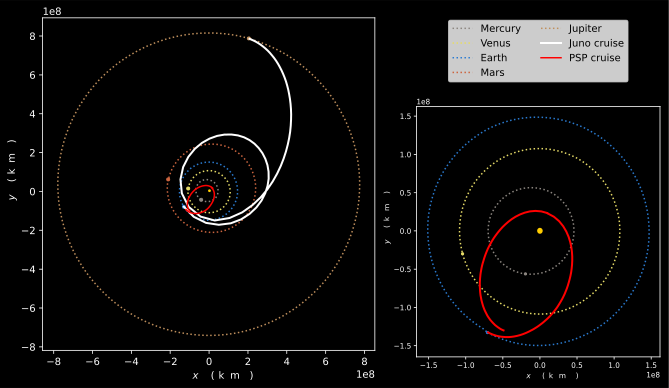
\includegraphics{images/orbits/juno_psp_orbit_v2.pdf}

}

\caption{Orbits}

\end{figure}%%
\begin{marginfigure}

{\centering {\marginnote{\begin{footnotesize}\includegraphics{index_files/mediabag/examples_Going_to_Ju.png}\end{footnotesize}}}

}

\caption{Previous Juno orbit using \texttt{poliastro}}

\end{marginfigure}%

\subsubsection{Discontinuities observed by different
spacecrafts}\label{discontinuities-observed-by-different-spacecrafts}

Juno, Parker Solar Probe, Wind and Stereo.

\begin{figure}

\begin{minipage}[t]{0.50\linewidth}

\raisebox{-\height}{

\includegraphics{./images/examples/fig-psp_id_example.pdf}

}

\subcaption{\label{}A RD detected by PSP at 0.126~AU}
\end{minipage}%
%
\begin{minipage}[t]{0.50\linewidth}

\raisebox{-\height}{

\includegraphics{index_files/mediabag/fig-juno_id_example.png}

}

\subcaption{\label{}A RD detected by Juno at 4 AU}
\end{minipage}%
\newline
\begin{minipage}[t]{0.50\linewidth}

\raisebox{-\height}{

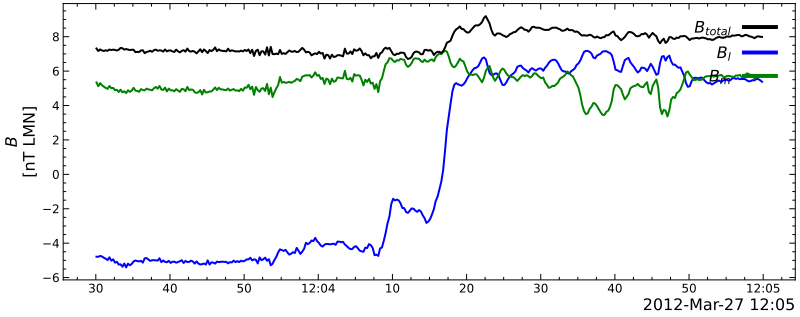
\includegraphics{./images/examples/fig-artemis_id_example.pdf}

}

\subcaption{\label{}A RD detected by ARTEMIS at 1 AU near Earth}
\end{minipage}%
%
\begin{minipage}[t]{0.50\linewidth}

\raisebox{-\height}{

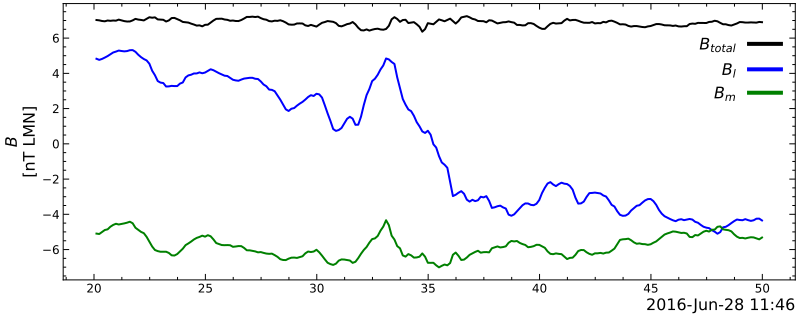
\includegraphics{./images/examples/fig-stereo_id_example.pdf}

}

\subcaption{\label{}A RD detected by STEREO at 1 AU at different solar
longitudes}
\end{minipage}%

\caption{\label{fig-ids}Rotational discontinuities (RDs) detected by
PSP, Juno, Stereo and near-Earth satellite at different radial distances
and solar longitudes.}

\end{figure}%

\subsubsection{Occurrence rate of
discontinuities}\label{occurrence-rate-of-discontinuities}

\includegraphics{index_files/mediabag/ocr_time_cleaned.png}

\subsubsection{Model validation}\label{model-validation}

We are using \href{http://csem.engin.umich.edu/MSWIM2D/}{Michigan Solar
WInd Model 2D (MSWIM2D)}, which models the solar wind propagation in 2D
using the BATSRUS MHD solver. (Keebler et al. 2022)

\begin{figure}[H]

{\centering \includegraphics{index_files/mediabag/juno_model_validatio.png}

}

\caption{Time-series comparison of MSWIM2D (red) and Juno-observed solar
wind}

\end{figure}%%
\begin{marginfigure}

{\centering {\marginnote{\begin{footnotesize}\includegraphics{images/paste-3.png}\end{footnotesize}}}

}

\caption{Time-series comparison of MSWIM2D (red) and New Horizons
SWAP-observed solar wind}

\end{marginfigure}%

\subsubsection{Solar wind properties}\label{solar-wind-properties}

\begin{figure}[H]

{\centering \includegraphics{index_files/mediabag/thickness_mn_dist.png}

}

\caption{Current sheet thickness}

\end{figure}%

\newpage{}

\subsection{Significance of Investigation \& Expected
Impact}\label{significance-of-investigation-expected-impact}

\subsection{Science Objectives and
Methodology}\label{science-objectives-and-methodology}

\subsection{Demonstration of Project
Approaches}\label{demonstration-of-project-approaches}

\subsubsection{Dataset, spacecraft instruments, and solar wind
model}\label{dataset-spacecraft-instruments-and-solar-wind-model}

Synergistic observations (Velli et al. 2020) advance our understanding
of the solar wind

\paragraph{Parker Solar Probe (PSP)}

\begin{itemize}
\tightlist
\item
  Links:
  \href{https://www.wikiwand.com/en/Parker_Solar_Probe}{Wikipedia}
\item
  (Fox et al. 2016; Raouafi 2022)
\item
  FIELDS (Bale et al. 2016) FIELDS Instrument Suite

  \begin{itemize}
  \tightlist
  \item
    About:: The FIELDS investigation will make direct measurements of
    electric and magnetic fields, the properties of in situ plasma
    waves, electron density and temperature profiles, and interplanetary
    radio emissions, amongst other things. The FIELDS instrument suite
    consists of two fluxgate magnetometers (MAG), three electric field
    antennas (EFS), and a waveform capture system (WAVES) that records
    the high frequency electric and magnetic waveforms at 16 samples per
    second.

    \begin{itemize}
    \item
      \begin{quote}
      The FIELDS experiment (Bale et al.~2016) measures magnetic and
      electric fields and their fluctuations in situ, and indirectly
      determines the electron density via plasma quasi-thermal noise
      spectroscopy. The investigation comprises two fluxgate
      magnetometers (MAG), a search coil magnetometer (SCM), and five
      electric antennas.
      \end{quote}
    \end{itemize}
  \end{itemize}
\item
  Solar Wind Electrons Alphas and Protons (SWEAP) Investigation (Kasper
  et al. 2016)

  \begin{itemize}
  \tightlist
  \item
    About:: a four sensor instrument suite that provides complete
    measurements of the electrons and ionized helium and hydrogen that
    constitute the bulk of solar wind and coronal plasma.
  \end{itemize}
\end{itemize}

\url{https://psp-gateway.jhuapl.edu/website/Home/psp_hci.mp4}

\url{https://psp-gateway.jhuapl.edu/website/Home/psp_hgmag.mp4}

\paragraph{Juno}

(Bolton et al. 2017)

\begin{itemize}
\tightlist
\item
  Magnetic Field investigation (MAG) (Connerney et al. 2017)

  \begin{itemize}
  \tightlist
  \item
    About:: The Juno Magnetic Field investigation (MAG) characterizes
    Jupiter's planetary magnetic field and magnetosphere, providing the
    first globally distributed and proximate measurements of the
    magnetic field of Jupiter. The magnetic field instrumentation
    consists of two independent magnetometer sensor suites, each
    consisting of a tri-axial Fluxgate Magnetometer (FGM) sensor and a
    pair of co-located imaging sensors mounted on an ultra-stable
    optical bench.
  \item
    Links:
    \href{https://www.wikiwand.com/en/Magnetometer_(Juno)}{Wikipedia},
    \href{https://doi.org/10.1007/s11214-017-0334-z}{DOI}
  \end{itemize}
\end{itemize}

\paragraph{Solar Orbiter (SO)}

Müller et al. (2020)

\begin{itemize}
\tightlist
\item
  In-situ instruments: -- Magnetometer (MAG, Horbury et al.~2020a) --
  Energetic Particle Detector (EPD, Rodríguez-Pacheco et al.~2020) --
  Radio and Plasma Wave analyser (RPW, Maksimovic et al.~2020a) -- Solar
  Wind Analyser (SWA, Owen et al.~2020)
\end{itemize}

\paragraph{Wind}

\begin{itemize}
\tightlist
\item
  About:: Comprehensive Solar Wind Laboratory for Long-Term Solar Wind
  Measurements
\item
  Instruments:

  \begin{itemize}
  \tightlist
  \item
    Magnetic Field Investigation (MFI) (Lepping et al. 1995)
  \item
    Solar Wind Experiment (SWE) (Ogilvie et al. 1995)
  \end{itemize}
\end{itemize}

\paragraph{Stereo}

\paragraph{ARTEMIS}

\subsubsection{Determination of
discontinuities}\label{determination-of-discontinuities}

Figures

\subsection{Relevance to Heliophysics Overarching
Goals}\label{relevance-to-heliophysics-overarching-goals}

\subsection{Project Schedule}\label{project-schedule}

\subsection{Management}\label{management}

\newpage{}

\section{Open Science and Data Management Plan
(OSDMP)}\label{open-science-and-data-management-plan-osdmp}

\begin{tcolorbox}[enhanced jigsaw, breakable, colframe=quarto-callout-note-color-frame, colback=white, titlerule=0mm, left=2mm, leftrule=.75mm, opacitybacktitle=0.6, coltitle=black, title=\textcolor{quarto-callout-note-color}{\faInfo}\hspace{0.5em}{Note}, bottomtitle=1mm, toprule=.15mm, arc=.35mm, toptitle=1mm, rightrule=.15mm, opacityback=0, colbacktitle=quarto-callout-note-color!10!white, bottomrule=.15mm]

This no-longer than two page section describes how any data, data
products and software created will be made public. An OSDMP, or an
explanation of why one is not needed given the nature of the work
proposed, is required. See Section 3.2.2 for instructions on what to
include.

\begin{itemize}
\tightlist
\item
  Length: 2 pages
\item
  Content: See Section II(c) for content and links to templates.
\end{itemize}

\end{tcolorbox}

\section{Research Readiness
Statement}\label{research-readiness-statement}

\begin{tcolorbox}[enhanced jigsaw, breakable, colframe=quarto-callout-note-color-frame, colback=white, titlerule=0mm, left=2mm, leftrule=.75mm, opacitybacktitle=0.6, coltitle=black, title=\textcolor{quarto-callout-note-color}{\faInfo}\hspace{0.5em}{Note}, bottomtitle=1mm, toprule=.15mm, arc=.35mm, toptitle=1mm, rightrule=.15mm, opacityback=0, colbacktitle=quarto-callout-note-color!10!white, bottomrule=.15mm]

This section consists of a research readiness statement of up to one
page authored by the FI that must include (a) and (b) conforming to
formatting requirements (line spacing, etc.) described above.

\begin{enumerate}
\def\labelenumi{\alph{enumi}.}
\tightlist
\item
  State and describe how the FI's undergraduate and/or graduate degree
  program and interactions with the mentor(s) prepare, or will prepare,
  the FI for the proposed research. Some possible questions to address
  include (but are not limited to): has the FI's past, current, and/or
  planned coursework and selfdirected study given the FI a good
  foundational understanding of the general subject area related to the
  proposed research? If a particular computer programming language,
  statistical analysis tool, experimental technique is required for the
  proposed project, is the FI proficient or has a plan to become
  proficient?
\item
  Provide a graduate study timeline that states i) the degree type
  (Ph.D., Master's, both, or other type of graduate degree, e.g., M.D.);
  ii) the subject area, iii) how long the FI has been (or if not yet
  admitted, expects to be) enrolled in the program, and iv) the
  estimated graduation date in Month/Year format.
\end{enumerate}

Part (c) should be included as appropriate, and should conform to
formatting requirements (line spacing, etc.) described above:

\begin{enumerate}
\def\labelenumi{\alph{enumi}.}
\setcounter{enumi}{2}
\tightlist
\item
  State and describe other experiences and/or self-directed learning
  activities that are relevant to the proposed research. This includes,
  but is not limited to, short courses offered at conferences,
  summer/winter schools, independent research projects, internships,
  work experience, volunteer experience, or teaching experience.
\end{enumerate}

\end{tcolorbox}

\paragraph{Professional preparation}\label{professional-preparation}

Zijin Zhang has taken fundamental physics courses (Electromagnetic
Theory, Plasma Physics, etc.) and space physics courses (Introduction to
Space Physics, Space Plasma Physics, and Solar System
Magnetohydrodynamics, etc.). He has conducted studies about\ldots{}
These courses and previous experience provide a good fundamental
understanding of the solar system and plasma waves. He is able to
analyze satellite data using IDL (SPEDAS), MATLAB, and Python.

\paragraph{Graduate study timeline}\label{graduate-study-timeline}

\begin{enumerate}
\def\labelenumi{\roman{enumi})}
\tightlist
\item
  Degree type:
\item
  Admitted date:
\item
  Time enrolled in the program: 3 years.
\item
  Estimated graduation date:
\end{enumerate}

\paragraph{Research experiences}\label{research-experiences}

\section{Biographical Sketches/Curriculum Vitae
(CVs)}\label{biographical-sketchescurriculum-vitae-cvs}

\subsection{Zijin's CV}\label{zijins-cv}

\subsection{Anton's CV}\label{antons-cv}

\section{Current and Pending Support}\label{current-and-pending-support}

\begin{tcolorbox}[enhanced jigsaw, breakable, colframe=quarto-callout-note-color-frame, colback=white, titlerule=0mm, left=2mm, leftrule=.75mm, opacitybacktitle=0.6, coltitle=black, title=\textcolor{quarto-callout-note-color}{\faInfo}\hspace{0.5em}{Note}, bottomtitle=1mm, toprule=.15mm, arc=.35mm, toptitle=1mm, rightrule=.15mm, opacityback=0, colbacktitle=quarto-callout-note-color!10!white, bottomrule=.15mm]

Current and Pending (C\&P) Support has no page limits. FIs must
identify, when applicable, any external-to-the-proposing organization
funding, e.g., from U.S. federal, U.S. non-federal, and non-U.S. sources
or active applications for grants, fellowships etc., particularly those
that have overlap with the proposed work. All PIs, regardless of F.5-14
the time devoted to FINESST, likewise must report C\&P. There is no
template established for reporting this information and if the reviewing
Division has a template posted, such templates may be used, but are not
required. C\&P templates or forms in use by the proposing institution
are welcome. To make it clear to NASA when the FI and/or PI have no C\&P
to report, include a joint statement or separate statements, if
applicable, that there is ``No C\&P funding to report''.

\end{tcolorbox}

\section{Statements of Commitment and Letters of Resource
Support}\label{statements-of-commitment-and-letters-of-resource-support}

\begin{tcolorbox}[enhanced jigsaw, breakable, colframe=quarto-callout-note-color-frame, colback=white, titlerule=0mm, left=2mm, leftrule=.75mm, opacitybacktitle=0.6, coltitle=black, title=\textcolor{quarto-callout-note-color}{\faInfo}\hspace{0.5em}{Note}, bottomtitle=1mm, toprule=.15mm, arc=.35mm, toptitle=1mm, rightrule=.15mm, opacityback=0, colbacktitle=quarto-callout-note-color!10!white, bottomrule=.15mm]

Do not add Statements of Commitment from any team member listed under
Section VI of the NSPIRES cover page and who acknowledges commitment via
NSPIRES. For example, when a collaborator or Co-I directly confirms
their participation via NSPIRES, that is sufficient commitment. If the
proposing team has regular access to a facility or resource, then no
letter of Resource support is needed. See Section 2.17 in the 2023 NASA
Proposer's Guide for how to prepare ``Letters of Resource Support'\,' to
demonstrate that a facility or resource is available for the proposed
use. Statements of commitment are only required when commitment cannot
be made via NSPIRES, such as when a proposer is using Grants.gov.

\end{tcolorbox}

\section{Mentoring Plan or Agreement}\label{mentoring-plan-or-agreement}

\begin{tcolorbox}[enhanced jigsaw, breakable, colframe=quarto-callout-note-color-frame, colback=white, titlerule=0mm, left=2mm, leftrule=.75mm, opacitybacktitle=0.6, coltitle=black, title=\textcolor{quarto-callout-note-color}{\faInfo}\hspace{0.5em}{Note}, bottomtitle=1mm, toprule=.15mm, arc=.35mm, toptitle=1mm, rightrule=.15mm, opacityback=0, colbacktitle=quarto-callout-note-color!10!white, bottomrule=.15mm]

\%• Mentoring Plan or Agreement - up to 2 pages. Exception: If the
submitting institution has a standard Mentor-Mentee checklist, plan,
agreement, template, etc., and it is longer than 2-pages, uses font
size, margins, etc., that do conform to this solicitation, then the
institution's standard is acceptable.

\%This section should not exceed two pages, except in the exception
noted below. The Mentoring Plan/Agreement's purpose is to provide the FI
with a holistic plan for developing skills and acquiring knowledge and
experience necessary to complete the research project and/or personal
professional development. This plan is reviewed under the research
readiness criterion from Section 5.1. This mentoring plan does not need
to re-state information provided in response to Sections 4.1.1 - 4.1.4.
The mentor(s) may explain in the mentoring plan why they have agreed to
support this FI's research. See also Section 12.20.

\%Both the FI and mentor prepare this agreement. It may include more
than one mentor; however, having additional mentors does not extend the
page limit. Non-PI mentors do not have to be at the submitting
institution. It is optional to include mentors beyond the PI, but if
they are named, they must be added to the NSPIRES cover page as team
members and must confirm their participation via NSPIRES.

\%The content, format, and organization of the mentoring plan are at the
discretion of the PI-FI team.

\end{tcolorbox}

\section{Budget Narrative (Budget
Justification)}\label{budget-narrative-budget-justification}

\section{References}\label{references}

\begin{itemize}
\tightlist
\item
  \href{https://parkersolarprobe.jhuapl.edu/The-Mission/index.php}{Parker
  Solar Probe: The Mission}
\end{itemize}

\phantomsection\label{refs}
\begin{CSLReferences}{1}{0}
\bibitem[\citeproctext]{ref-bale2016}
Bale, S. D., K. Goetz, P. R. Harvey, P. Turin, J. W. Bonnell, T.
Dudok~de~Wit, R. E. Ergun, et al. 2016. {``The FIELDS Instrument Suite
for Solar Probe Plus.''} \emph{Space Science Reviews} 204 (1): 49--82.
\url{https://doi.org/10.1007/s11214-016-0244-5}.

\bibitem[\citeproctext]{ref-bolton2017}
Bolton, S. J., J. Lunine, D. Stevenson, J. E. P. Connerney, S. Levin, T.
C. Owen, F. Bagenal, et al. 2017. {``The Juno Mission.''} \emph{Space
Science Reviews} 213 (November): 5--37.
\url{https://doi.org/10.1007/s11214-017-0429-6}.

\bibitem[\citeproctext]{ref-connerney2017}
Connerney, J. E. P., M. Benn, J. B. Bjarno, T. Denver, J. Espley, J. L.
Jorgensen, P. S. Jorgensen, et al. 2017. {``The Juno Magnetic Field
Investigation.''} \emph{Space Science Reviews} 213 (1): 39--138.
\url{https://doi.org/10.1007/s11214-017-0334-z}.

\bibitem[\citeproctext]{ref-fox2016}
Fox, N. J., M. C. Velli, S. D. Bale, R. Decker, A. Driesman, R. A.
Howard, J. C. Kasper, et al. 2016. {``The Solar Probe Plus Mission:
Humanity{'}s First Visit to Our Star.''} \emph{Space Science Reviews}
204 (1): 7--48. \url{https://doi.org/10.1007/s11214-015-0211-6}.

\bibitem[\citeproctext]{ref-kasper2016}
Kasper, Justin C., Robert Abiad, Gerry Austin, Marianne Balat-Pichelin,
Stuart D. Bale, John W. Belcher, Peter Berg, et al. 2016. {``Solar Wind
Electrons Alphas and Protons (SWEAP) Investigation: Design of the Solar
Wind and Coronal Plasma Instrument Suite for Solar Probe Plus.''}
\emph{Space Science Reviews} 204 (1): 131--86.
\url{https://doi.org/10.1007/s11214-015-0206-3}.

\bibitem[\citeproctext]{ref-keebler2022}
Keebler, Timothy B., Gábor Tóth, Bertalan Zieger, and Merav Opher. 2022.
{``MSWIM2D: Two-Dimensional Outer Heliosphere Solar Wind Modeling.''}
\emph{The Astrophysical Journal Supplement Series} 260 (2): 43.
\url{https://doi.org/10.3847/1538-4365/ac67eb}.

\bibitem[\citeproctext]{ref-lepping1995}
Lepping, R. P., M. H. Acũna, L. F. Burlaga, W. M. Farrell, J. A. Slavin,
K. H. Schatten, F. Mariani, et al. 1995. {``The WIND Magnetic Field
Investigation.''} \emph{Space Science Reviews} 71 (1): 207--29.
\url{https://doi.org/10.1007/BF00751330}.

\bibitem[\citeproctext]{ref-muxfcller2020}
Müller, D., O. C. St Cyr, I. Zouganelis, H. R. Gilbert, R. Marsden, T.
Nieves-Chinchilla, E. Antonucci, et al. 2020. {``The Solar Orbiter
Mission - Science Overview.''} \emph{Astronomy \& Astrophysics} 642
(October): A1. \url{https://doi.org/10.1051/0004-6361/202038467}.

\bibitem[\citeproctext]{ref-ogilvie1995}
Ogilvie, K. W., D. J. Chornay, R. J. Fritzenreiter, F. Hunsaker, J.
Keller, J. Lobell, G. Miller, et al. 1995. {``SWE, a Comprehensive
Plasma Instrument for the WIND Spacecraft.''} \emph{Space Science
Reviews} 71 (1): 55--77. \url{https://doi.org/10.1007/BF00751326}.

\bibitem[\citeproctext]{ref-raouafi2022}
Raouafi, Nour E. 2022. {``A Journey to Touch the Sun.''} \emph{Physics
Today} 75 (11): 28--34. \url{https://doi.org/10.1063/PT.3.5120}.

\bibitem[\citeproctext]{ref-velli2020}
Velli, M., L. K. Harra, A. Vourlidas, N. Schwadron, O. Panasenco, P. C.
Liewer, D. Müller, et al. 2020. {``Understanding the Origins of the
Heliosphere: Integrating Observations and Measurements from Parker Solar
Probe, Solar Orbiter, and Other Space- and Ground-Based
Observatories.''} \emph{Astronomy and Astrophysics} 642 (October): A4.
\url{https://doi.org/10.1051/0004-6361/202038245}.

\end{CSLReferences}



\end{document}
